\documentclass[main.tex]{subfiles}
\begin{document}

\subsection{Ángulos de Euler (Roll-Pitch-Yaw)}
\begin{figure}[h]
  \centering
  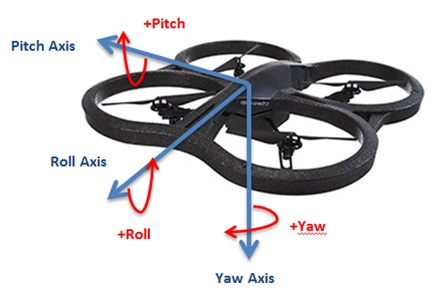
\includegraphics[width=0.3\textwidth]{../img/rpy_drone.jpg}
  \caption{Drone con sus ejes de Euler}
  \label{rpy_drone}
\end{figure}

\begin{itemize}
\item Conversión a matriz de rotación
  \begin{equation}
    \label{eq:matriz_Rot}
    R = R_{Z}(\psi) * R_{Y}(\theta) * R_{X}(\phi)
  \end{equation}
  Donde:
  \begin{equation}
    \label{eq:matriz_Rz}
    R_{Z}(\psi) = \begin{pmatrix}
          \cos \psi  & -\sin \psi  &0 \\ 
          \sin \psi &\cos \psi  & 0\\ 
          0&  0& 1
         \end{pmatrix}
  \end{equation}
  \begin{equation}
    \label{eq:matriz_Ry}
    R_{Y}(\theta) = \begin{pmatrix}
           \cos \theta&0&\sin \theta\\ 
           0 &1  &0 \\ 
           \sin \theta &0  & \cos \theta
         \end{pmatrix}
  \end{equation}
  \begin{equation}
    \label{eq:matriz_Rx}
    R_{X}(\phi) = \begin{pmatrix}
           1 &0  &0 \\ 
           0 &\cos \phi&-\sin \phi \\ 
           0 &\sin \phi&\cos \phi 
         \end{pmatrix}
  \end{equation}
%  Reemplazando (\ref{eq:matriz_Rz}),
%  (\ref{eq:matriz_Ry}),
%  (\ref{eq:matriz_Rx}) en
%  (\ref{eq:matriz_Rot}):
%  \begin{equation}
%    R = \bigl( \begin{bmatrix}
%            \cos\psi \cos\theta &
%            \cos\psi\sin\theta\sin\phi-sin\psi\cos\phi &
%            cos\psi\sin\theta\cos\phi+\sin\psi\sin\phi
%          \\
%            \sin\psi \cos\theta &
%            \sin\psi\sin\theta\sin\phi+cos\psi\cos\phi & 
%            \sin\psi\sin\theta\cos\phi-\cos\psi\sin\phi
%          \\
%            -\sin\theta &
%            \cos\theta\sin\phi  &
%            \cos\theta\cos\phi 
%        \end{bmatrix} \bigr)
%  \end{equation}
\item Conversión de matriz de rotación
  \begin{equation}
    \phi=\arctan 2(-r_{31},\sqrt{r_{11}^2+r_{21}^2})
  \end{equation}
  \begin{equation}
    \psi=-\arctan 2(\frac{r_{21}}{\cos\phi},\frac{r_{11}}{\cos\phi})
  \end{equation}
  \begin{equation}
    \theta=\arctan 2(\frac{r_{32}}{\cos\phi},\frac{r_{33}}{\cos\phi})
  \end{equation}
\end{itemize}

\subsection{Axis-Angle (eje-ángulo)}

\begin{figure}[h]
  \centering
  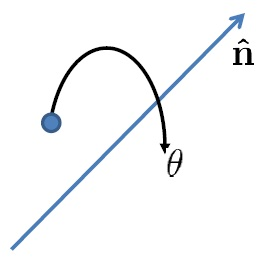
\includegraphics[width=0.25\textwidth]{../img/axisang.jpg}
  \caption{Ejemplo de Axis-angle}
  \label{axisang}
\end{figure}

Conversiones (Fórmula de Rodriguez)
\begin{equation}
  R(\hat{n},\theta) = I +
      \sin\theta\left [ \hat{n} \right ]_{x}
      +(1-\cos\theta)\left [ \hat{n} \right ]_{x}^2
\end{equation}
\begin{equation}
  \theta=\\cos^{-1}(\frac{trace(R)-1}{2})
\end{equation}
\begin{equation}
  \hat{n} = \frac{1}{2\sin\theta}
            \begin{bmatrix}
              r_{32}-r_{23}\\ 
              r_{13}-r_{31}\\ 
              r_{21}-r_{12}
            \end{bmatrix}
\end{equation}

\subsection{Quaterniones}
\begin{itemize}
\item Representación vectorial
  \begin{equation}
    q=\left ( q_{w},q_{x},q_{y},q_{z} \right )^T \in \mathbb{R}^4
  \end{equation}
  \begin{equation}
    q=\left ( r,v \right )^T  
  \end{equation}
\item Quaternion unitario
  \begin{equation}
    \left \| q \right \|=1
  \end{equation}
\item Relación Axis-angle
  \begin{equation}
    q = \left( r,v \right) ^ T
      = \left(
          \cos\frac{\theta}{2},
          \sin\frac{\theta}{2} \hat{n}
        \right) ^ T
  \end{equation}
\end{itemize}

\end{document}